\namedsection{Final Design}{Gupta}

The final layout of the hardware does indeed follow what was initially planned. As can be seen from figures~\ref{fig:hardware_schematic_development-2} and~\ref{fig:hardware_schematic_final-2} as compared to figures~\ref{fig:hardware_schematic_development} and~\ref{fig:hardware_schematic_final}, they are very similar except the actual protocols for communication have been determined. 

The LED for the mBed was straightforward to do and did not require any additional hardware due to the fact that the mBed has four user programmable LEDs on board, allowing for the desired visual output. It also permitted a few additional for an extra level of debugging, especially when the device is not connected to the host PC via the serial connection.

\begin{figure}
	\centering
	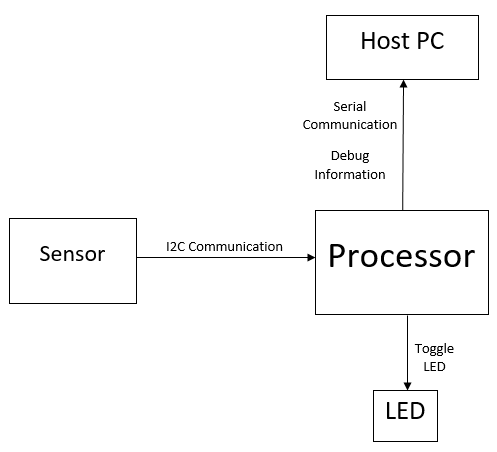
\includegraphics{hardware-schematics-development-2.pdf}
	\caption{Final Hardware Block Diagram - Development}
	\label{fig:hardware_schematic_development-2}
\end{figure}

\begin{figure}
	\centering
	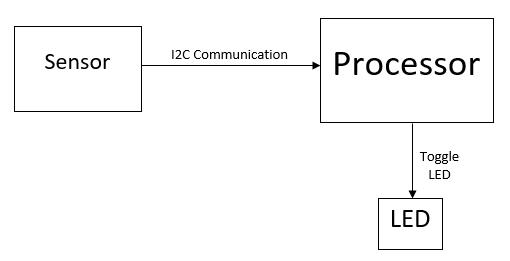
\includegraphics{hardware-schematics-final-2.pdf}
	\caption{Final Hardware Block Diagram - Final}
	\label{fig:hardware_schematic_final-2}
\end{figure}